\chapter{Methods}
After previous chapters we should achieve basic understanding of neural network models and physics. Now we study state of the art methods which should capture hamiltonian model on studied datasets. 
\section{New paradigm - NeuralODE}
Neural ODE is very interesting and important concept for solving the Ordinary Differential Equations and training the neural networks with trajectory data.\\
The default situation is described as:
\begin{equation}
	\dot{\mathbf{x}}=\mathbf{f}(\mathbf{x},t|\Theta)
\end{equation}
Where $\mathbf{f}(\mathbf{x},t|\Theta) $ represents the multilayer perception which creates vector field.
This method has its history from residual networks where their feed-forward network looks like euler step
\begin{equation}
	\mathbf{h}^{(i+1)} = \mathbf{h}^{(i)} + \mathbf{f}(\mathbf{h}^{(i)}|\Theta)
\end{equation}

In the paper \cite{neuralODE} it is introduced a adjoint method  which solves problem with vanishing gradients.\\
This is achieved trough continuous backpropagation which is stated in the paper.
We can compare it 
\begin{center}
	\begin{tabular}{ c c|c }
		 & residual network & adjoint method \\ 
		 \hline
		$a_t$ or $a(t)$: & $\frac{\partial L}{\partial z}$ & $\frac{\partial L}{\partial z(t)}$ \\  
		forward-pass: & $z_{i+1} = z_t + hf(z_t)$ & $z(t+1) = z(t)+\int_t^{t+1}f(t)dt$\\
		backward-pass: &$a_t = a_{t+1}+ha_{t+1}\frac{\partial f(z_t)}{\partial z_t}$ & $a(t) = a(t+1)+\int_{t+1}^ta(t)\frac{\partial f(z(t))}{\partial z(z)}dt$\\
		gradients:  & $\frac{\partial L}{\partial \theta}=ha_{t+h}\frac{\partial f(z(t),\Theta)}{\partial \Theta}$ & $\frac{\partial L}{\partial \theta}=\int_t^{t+1}a(t)\frac{f(z(t),\Theta)}{\partial \Theta}$   
	\end{tabular}
\end{center}
For PINN models the adjoint method over framework \texttt{torchdiffeq} doesn't work properly because of the computed gradients which PINNs produce. In case of PINN models we suggest to use normal rollout with ode solver like RK4.


\section{Recurrent time steppers}
In chapter \ref{background}  we introduced recurrent models which are RNN and GRU.
Those models are very good at learning the time series data. To make it more physics informed we applied an euler method which it makes to time stepper models:
\begin{eqnarray}
	[\mathbf{v}_i, \mathbf{h}_{i+1}] = \text{MLP}(\text{RNN}(\mathbf{x}_i,\mathbf{h}_i) \text{  or  }  \text{GRU}(\mathbf{x}_i,\mathbf{h}_i))\\
	\mathbf{x}_{i+1} = \mathbf{x}_i + \mathbf{v}_i \cdot dt
\end{eqnarray}
We describe it this procedure as a rollout. 
This model has one big static parameter dependency which is fixed $dt$. We suggest to not to change this parameter after training. In Chapter Experimentation we will show the performance of RNN and GRU time stepper models. In the figure \ref{fig:rnn} we can see the architecture of the model.
\begin{figure}[h!]
	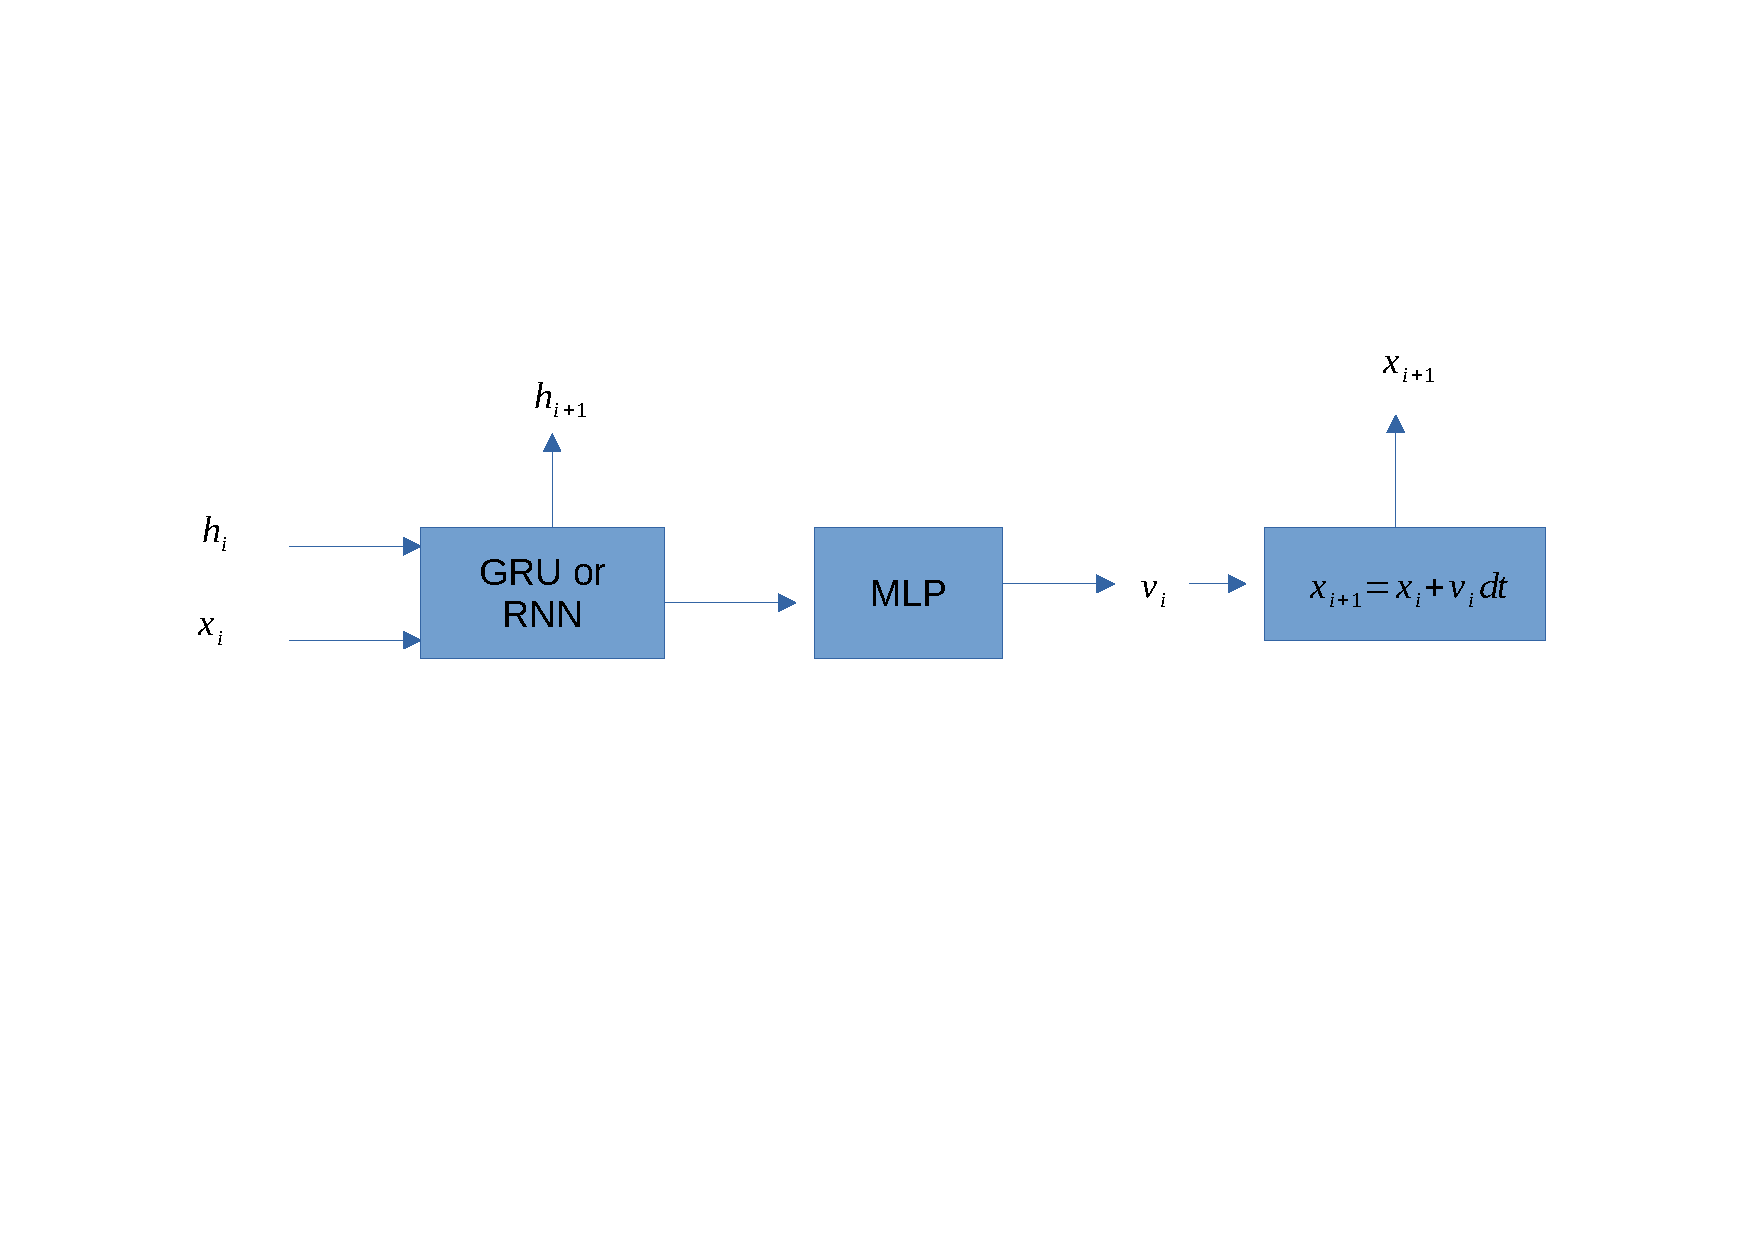
\includegraphics[width=15cm]{chapters/chapter4/GRU_stepper}
	
	\caption{Architecture of time-stepper model}
	\label{fig:rnn}
\end{figure}



\section{Hamiltonian Neural Network}
This model comes from the paper \cite{hnn} it is one of the physics informed models because it uses differentiation technique and applies the Hamiltonian equations. In this case the $\mathbf{x} = [\mathbf{q},\mathbf{p}]$ are canonical or natural coordinates(Cartesian space).
The forward pass looks like:
\begin{eqnarray}
	H_{\Theta} &=& \mathbf{f}(\mathbf{x}|\boldsymbol{\Theta})\\
	\frac{d\mathbf{x}}{dt}(\mathbf{x}) &=& \left[\frac{\partial H_{\Theta}}{\partial\mathbf{p}}(\mathbf{x}),-\frac{\partial H_{\Theta}}{\partial\mathbf{q}}(\mathbf{x})\right]^T
\end{eqnarray}
In the paper they train it only over the produced vectorfield.
For our experiments we made rollout part for the network to create trajectory. 
To make trajectory we use ODE solver
\begin{equation}
	\mathbf{x} = \text{odeint}\left(\frac{d\mathbf{x}}{dt},\mathbf{x}_0,t\right)
\end{equation} 
The odeint operator in this equation is a solver for ODEs like euler or RK4 method. We can observe it in the figure from chapter Introduction \ref{fig:hnn}.\\
\section{Graph Neural Network}
Graph neural Networks are very new neural architecture which is available today. It is used broadly in social sciences and in chemistry like generating new chemical compounds.\\
The main part of GNN is a graph $\mathbf{G}$. It is defined as a collection of vertices and edges $\mathbf{G}=\{\mathbf{V},\mathbf{E}\}$ where $\mathbf{V} = \{\mathbf{v}_1,...,\mathbf{v}_i,...,\mathbf{v}_n\}$ has $n$ vertices
and $\mathbf{E} = \{\mathbf{e}_1,...,\mathbf{e}_i,...,\mathbf{e}_m\}$
has $m$ edges.\\
The edge is connection between to nodes it can be directed(only one direction between the nodes) or undirected(both direction between the nodes). This is very important because the graphs has many properties which we can use building it as Graph Neural Model.\\
This connectivity can be represented with adjacency matrix $\mathbf{A}$.
Adjacency matrix is denoted as $\mathbf{A}\in \{0,1\}^{n x n}$ 
\begin{equation}
\mathbf{A}_{ij} =	\left\{\begin{matrix}
		1 & if (\mathbf{v}_i , \mathbf{v}_j)\in\mathcal{E}\\
		0 & otherwise
	\end{matrix}\right.
\end{equation}

Most important property of graphs is creating the normailzed Laplacian matrix. This is foundation of the idea about graph neural networks and it is defined as:
\begin{equation}
	\mathbf{L}= \mathbf{I} - \mathbf{D}^{\frac{1}{2}}\mathbf{A}\mathbf{D}^{\frac{1}{2}} 
\end{equation} where $\mathbf{D}$ is degree matrix. Degree of a node is the number of nodes that are adjecent to the node in question. This matrix has only diagonal elements.\\
In the figure \ref{graph} you can see a representation of the graph together with adjecency matrix.
\begin{figure}[h!]
	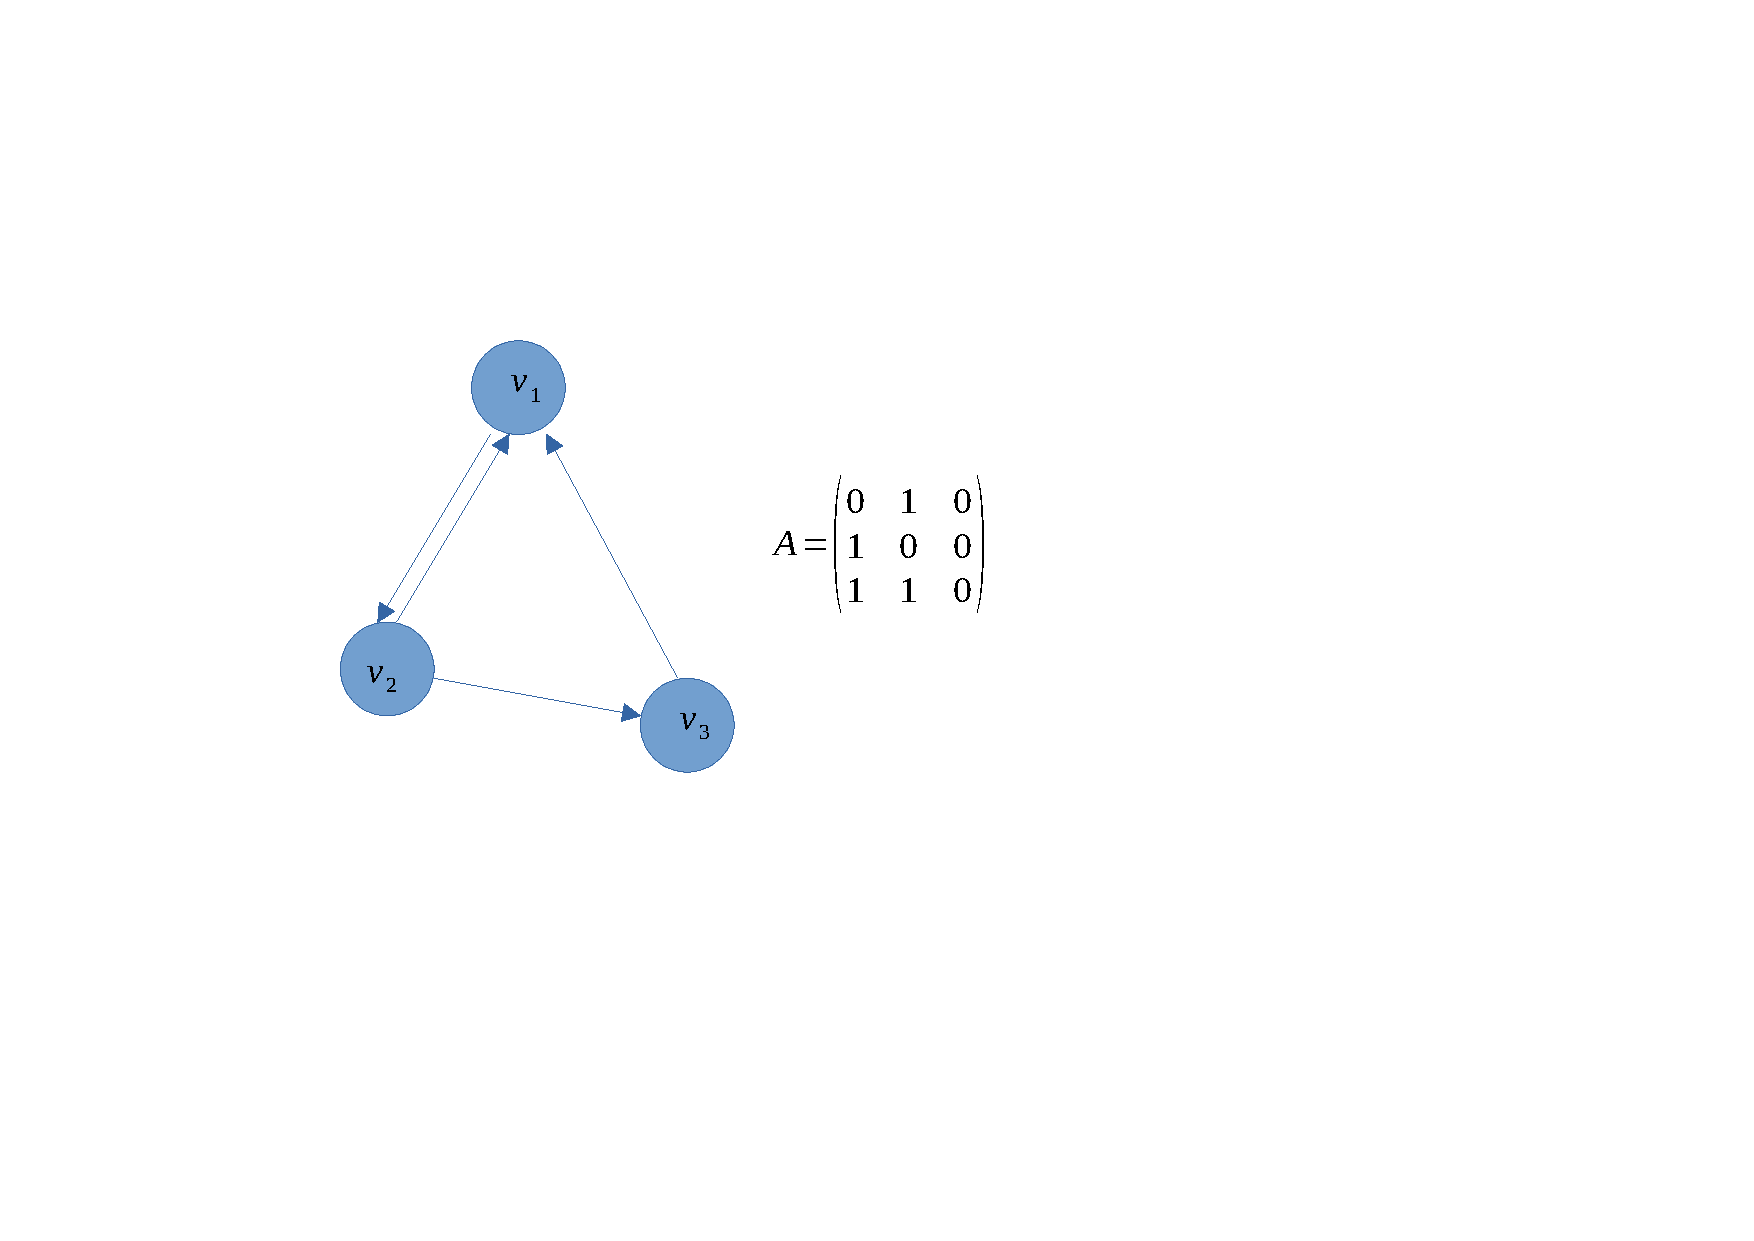
\includegraphics[width=15cm]{chapters/chapter4/graph}
	
	\caption{Graph representation}
	\label{graph}
\end{figure}
We recognize 3 main training types of GNNs and that are graph- , edge and node - oriented learning.\\
We will do only node oriented learning because we care that our data from the nodes comes dynamically right. For this we implemented two Graph Neural Layer to our work. 

\subsection{Convolutional Graph Neural Network}
First idea about graph neural network was Spectral Graph Network (SGN) \cite{sgn} in signal proccesing tasks which is based on spectrality of the modified  Laplacian in form \begin{equation}
	\mathbf{L}= \mathbf{I} - \mathbf{D}^{\frac{1}{2}}\mathbf{W}\mathbf{D}^{\frac{1}{2}} 
\end{equation}where we exchange adjecency matrix with learnable weight matrix.
Because of cost of computation and hard backpropagation, the ChebNet was introduced\cite{cheb}. 
It was dependent of fourier transformation and had high computational comlpexity.
First Kipf and Welling used both ideas and simplified Laplacian to create broadly used architecture called convolutional graph network \cite{gcn}. \\
The propagation of the layer mathematically looks like
\begin{equation}
	\mathbf{h}^{(i+1)}=\sigma(\tilde{\mathbf{D}}^{\frac{1}{2}}\tilde{\mathbf{A}}\tilde{\mathbf{D}}^{\frac{1}{2}}\mathbf{W}\mathbf{h}^{(i)})
\end{equation} where we modify adjacency matrix $\tilde{\mathbf{A}}=\mathbf{A}+ \mathbf{I}$ and $\tilde{\mathbf{D}}$ as $\tilde{\mathbf{D_{ij}}} =\sum_{j=1}^N \tilde{\mathbf{A}}_{ij}.$ 
This mathematical expression of propagation of the graph layer is equivalent to message passing on the  and aggregation on the graph from and between the neighbouring nodes. In this case with $\sum$ operator.\\ There are other types of aggregations like $\texttt{mean}$, $\texttt{sum}$ and $\texttt{sub}$. 
The default message passing and aggregation formula is defined as
\begin{equation}
\mathbf{x}_i^{(k)} = \gamma^{(k)} \left( \mathbf{x}_i^{(k-1)}, \bigoplus_{j \in \mathcal{N}(i)} \, \phi^{(k)}\left(\mathbf{x}_i^{(k-1)}, \mathbf{x}_j^{(k-1)},\mathbf{e}_{j,i}\right) \right) 
\end{equation} where $\gamma$ and $\phi$ represents MLPs and $\bigoplus$ the aggregation function. 
While the neural graph network doesn't depend on the graph structure itself, it relies on message passing and aggregation between the nodes. With this understanding, we can develop more diverse designs of graph neural networks. 
%With knowledge that the neural network doesn't depend on graph structure,on the other hand it depends on massage passing and aggregation between the nodes, we can build more designs of graph neural networks.\\ 
We should not forget, that those message passing and aggregation can be parallelized and calculated on GPUs improving performance. In our use cases we will use Framework \texttt{DGL}\cite{dgl}.


\subsection{Gated Attention Network}
In paper \cite{gat} is intoduced new type of architecture which incomporates weighting factors/attentional coefficients. This weightning factors $\alpha$ shows importance of the outgoing node  to the  ingoing node in question. 
The forward pass of one layer is defined as:
\begin{eqnarray}
\mathbf{z}_i^{(l)}&=&\mathbf{W}_f^{(l)}\mathbf{h}_i^{(l)}, \\
e_{ij}^{(l)}&=&\text{LeakyReLU}(\mathbf{W_a}^{(l)^T}(\mathbf{z}_i^{(l)}||\mathbf{z}_j^{(l)})),\\
\alpha_{ij}^{(l)}&=&\frac{\exp(e_{ij}^{(l)})}{\sum_{k\in \mathcal{N}(i)}^{}\exp(e_{ik}^{(l)})},\\
\mathbf{h}_i^{(l+1)}&=&\sigma\left(\sum_{j\in \mathcal{N}(i)} {\alpha^{(l)}_{ij} \mathbf{z}^{(l)}_j }\right)
\end{eqnarray}

This architecture is computationally efficient and  is applicable to inductive problems, thus the creation of weighting factors doesn't depend on global graph structure. We will have always one weighting factor per edge no matter which graph we use.%, furthermore the weightning factors are created one per edge within the multilayer perceptron. This means that the weightning factors are not bounded to the size of the graph and behaves dynamicly. % are not hard-coded and they are calculated in dependence with a graph structure.
For better training and preventing overfitting, we can set a dropout at MLP which creates weightning factors\cite{att}, it is even suggested for  the small graphs.












\section{Graph Hamiltonian Neural Network}
This architecture is inspired on implementation of HNN\cite{hnn} and paper \cite{GNNODE}. In the paper they implemented own Graph Neural Network with complicated architecture called GN, which has many applications in deep learning.  They tried this architecture incorporate with odeint solver to create HOGN model.
In our case we will use conventional GNN model to create the same.
In our cases our graph will built without loop nodes: Nodes with edge connected itself. With many trials we achieve same valued features at the nodes using \texttt{sum} or \texttt{mean} aggregation at fully connected graph, With discarding self loops we don't have this problem anymore.\\  It is important that the output of our Graph network is a scalar value because it represents $\mathcal{H}$. Without this condition, auto differentiation won't work. 
There is the forumla for GHNN.
\begin{eqnarray}
	H_{\Theta} &=& \mathbf{f}(\mathbf{x}|\boldsymbol{\Theta})=\text{GNN layer }(\mathbf{x})\\
	\frac{d\mathbf{x}}{dt} &=& \left[\frac{\partial H_{\Theta}}{\partial\mathbf{p}}(\mathbf{x}),-\frac{\partial H_{\Theta}}{\partial\mathbf{q}}(\mathbf{x})\right]^T
\end{eqnarray}
The Graph Neural Network can be made with more layers and we can add activation functions. In the experiments we used GAT layer.\\
This model gives trajectory trough using of one ode solvers. Its architecture you can observe in Figure \ref{ghnn}.
\begin{figure}[h!]
	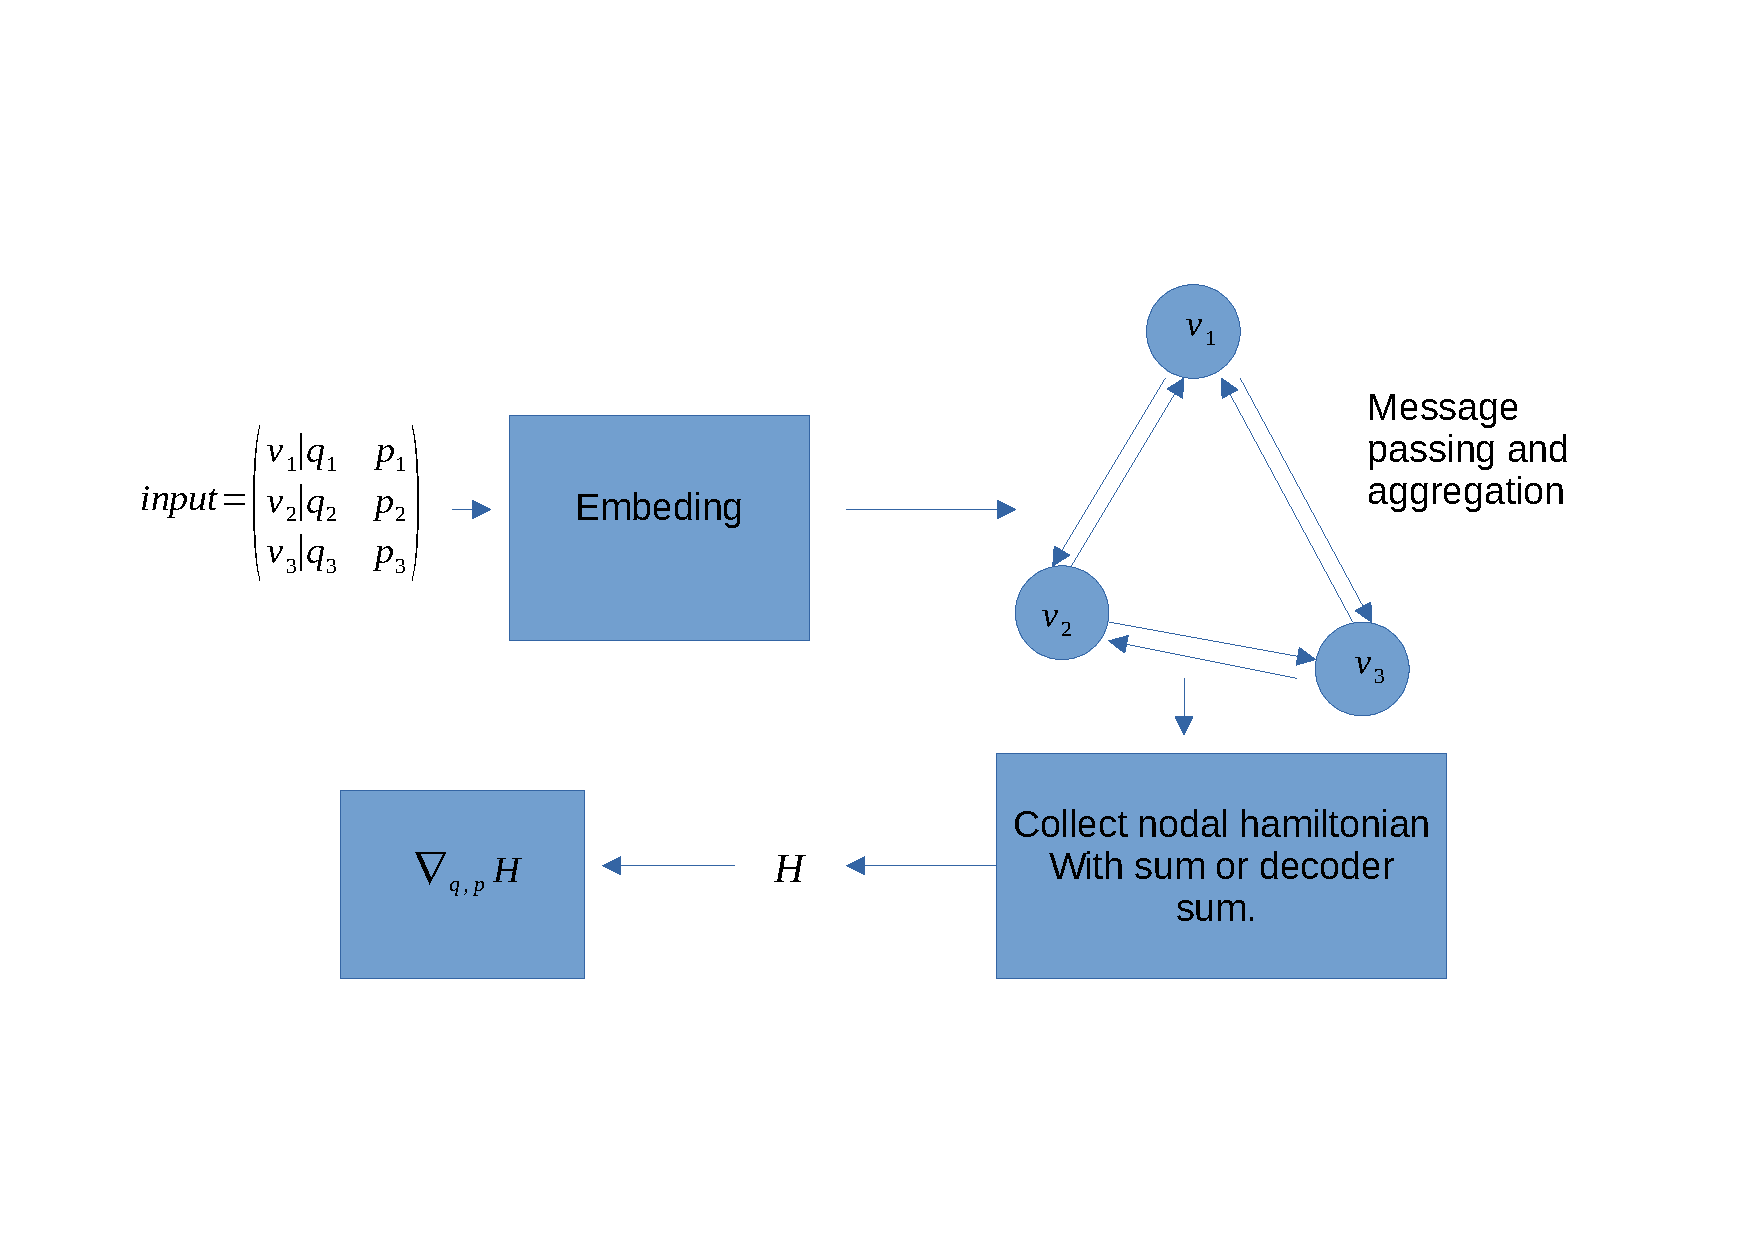
\includegraphics[width=15cm]{chapters/chapter4/ghnn}
	\caption{Architecture of Graph Neural Hamiltonian Network}
	\label{ghnn}
\end{figure}
\section{Improved Graph Hamiltonian Neural Network}
As GHNN mentioned before didn't showed  very good performance we were forced to find some new architecture. We found new layer which we could use and it is inspired by paper \cite{wave}. The adapting adjecency matrix is very interesting concept but in the scope of coding, the \texttt{DGL} don't allow fitting the adjecency matrix.\\
In the paper adaptive adjecency matrix was calculated as
\begin{equation}
	\mathbf{A_{adp}} = Softmax(ReLU(\mathbf{E_1}\mathbf{E_2^T})),
\end{equation}
This procedure looks very alike attentional coefficient calculation.
We made our architecture for one layer as

\begin{eqnarray}
	\mathbf{y}_{gcn} &=& GCN(\mathbf{x}),\\
	\mathbf{y}_{gat} &=& GAT(\mathbf{x}),\\
	\mathbf{y}_{mlp} &=& MLP(\mathbf{y}_{gcn}|\mathbf{y}_{gat}),\\
	\mathbf{y} &=& \mathbf{y}_{gcn}+\mathbf{y}_{gat}+\mathbf{y}_{mlp}\\
	H_{\Theta} &=& \sum \mathbf{y} \text{   sum of the all features}\\
	\frac{d\mathbf{x}}{dt} &=& \left[\frac{\partial H_{\Theta}}{\partial\mathbf{p}}(\mathbf{x}),-\frac{\partial H_{\Theta}}{\partial\mathbf{q}}(\mathbf{x})\right]^T
\end{eqnarray}
We used the multilayer perceptron as some sort of decoder which uses concatenated input of outputs from GAT and GCN layer. After that we sum everything together.\\
We will use it in some of our experiments. The architecture can be observed in Figure \ref{improvedGHNN}

\begin{figure}[h!]
	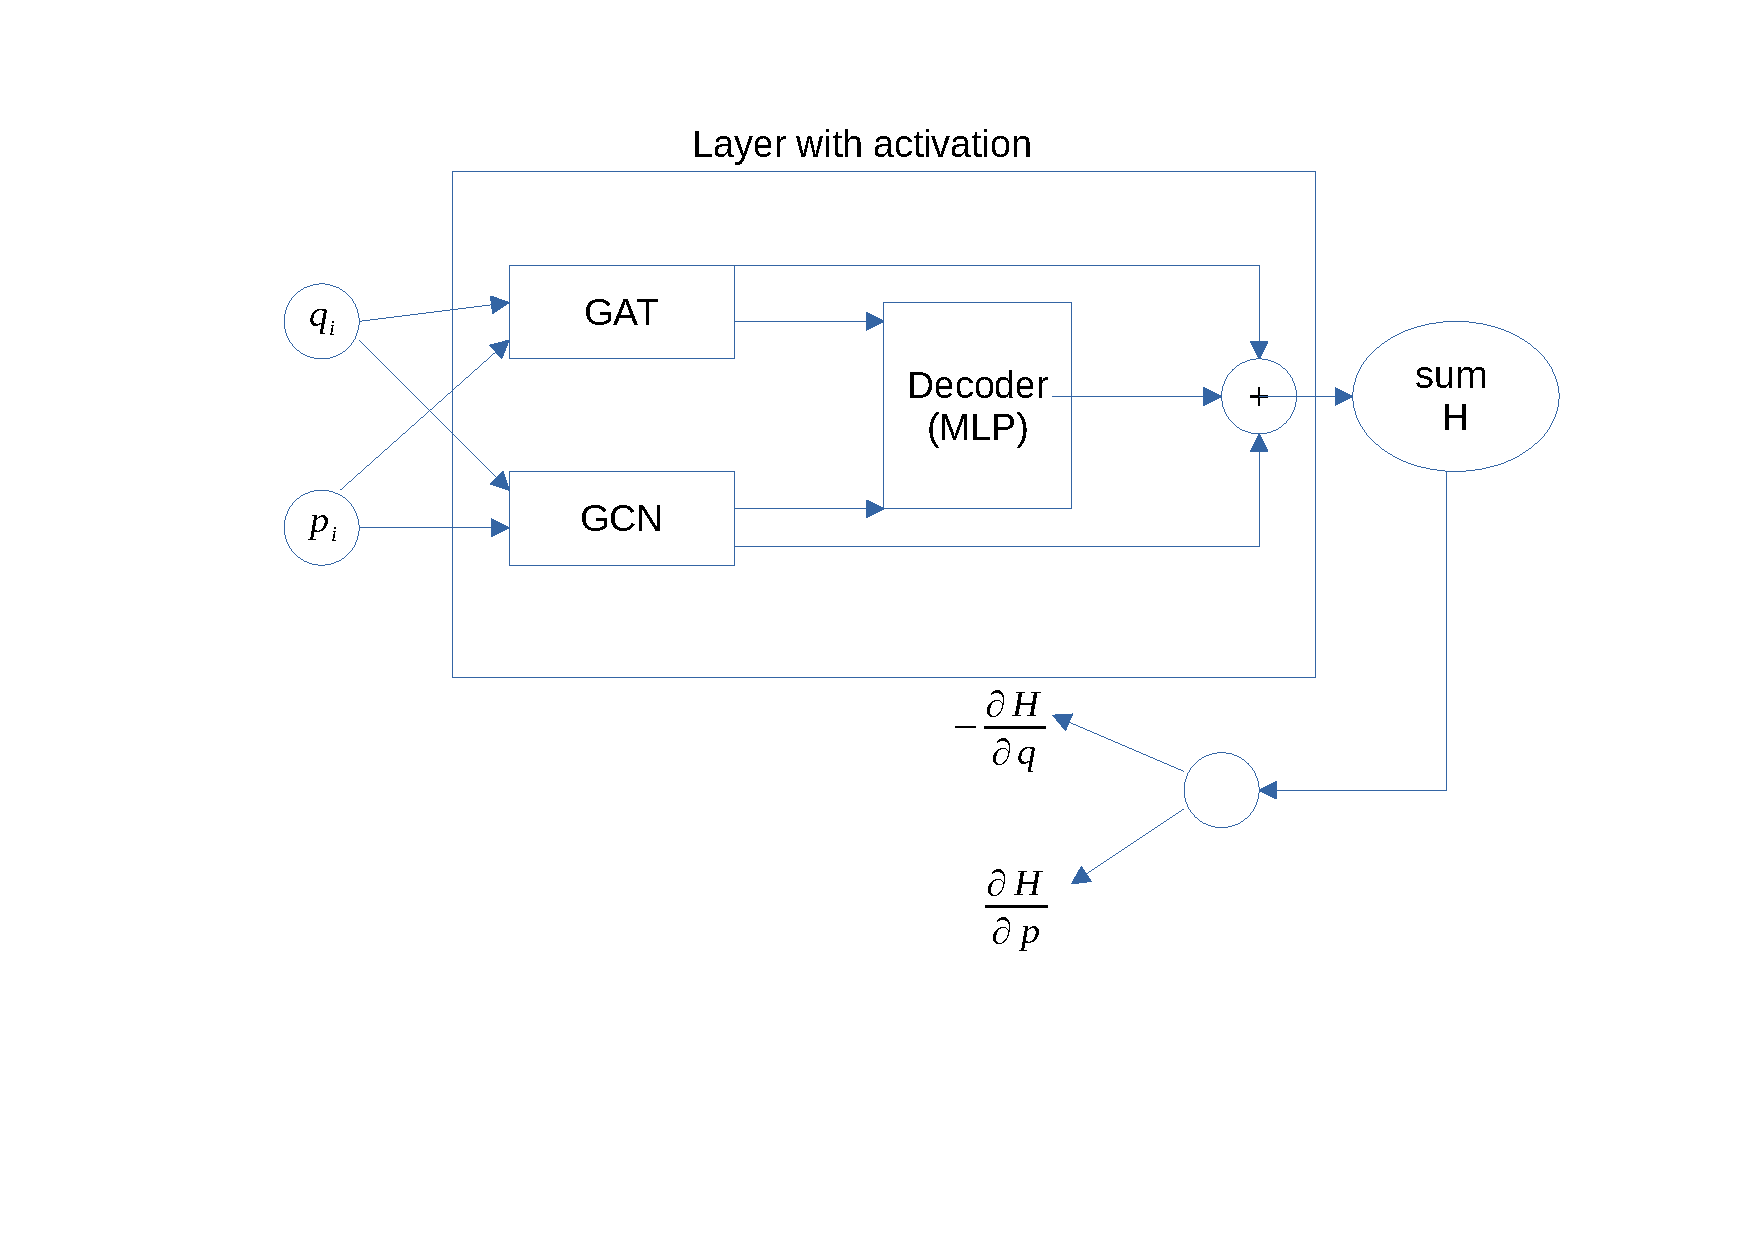
\includegraphics[width=15cm]{chapters/chapter4/improved_GHNN.pdf}
	
	\caption{Architecture of improved GHNN}
	\label{improvedGHNN}
\end{figure}
This architecture shows better performance then GHNN, but it is relatively slow. 
 

 



\section{Gated Recurrent Graph Hamiltonian Neural Network - GRUGHNN}
In previous section we introduced the GHNN, which is base an Hamiltonian layer and ode-solver. This architecture is not different but improved with a GRU unit at the beginning of the input. this model is equivalent to the GRU stepper but we added a GHNN in it. It is Graph Neural Network with a memory feature. If we compare this model to spatio-temporal models you can see similarities. Only two models have similar architecture to this. We will mention Gated Graph Sequence Neural Network\cite{GGSNN} and GNN-GRU\cite{gnngru}, but they don't use auto differentiation. Without autodifferentiation we can not call our architectures as "hamiltonian". 

\begin{eqnarray}
	[\mathbf{a}_i, \mathbf{h}_{i+1}] &=&  \text{GRU}(\mathbf{x}_i,\mathbf{h}_i)\\
	 H_i&=& \text{GNN}(\mathbf{a}_i)\\
	 \mathbf{v}_i&=&\left[\frac{\partial H_{i}}{\partial\mathbf{p}}(\mathbf{x}),-\frac{\partial H_{i}}{\partial\mathbf{q}}(\mathbf{x})\right]^T\\
	 \mathbf{x}_{i+1} &=& \mathbf{x}_i + \mathbf{v}_i \cdot dt
\end{eqnarray}
Architecture of our network you can observe in Figure \ref{GRUGHNN}
\begin{figure}[h!]
	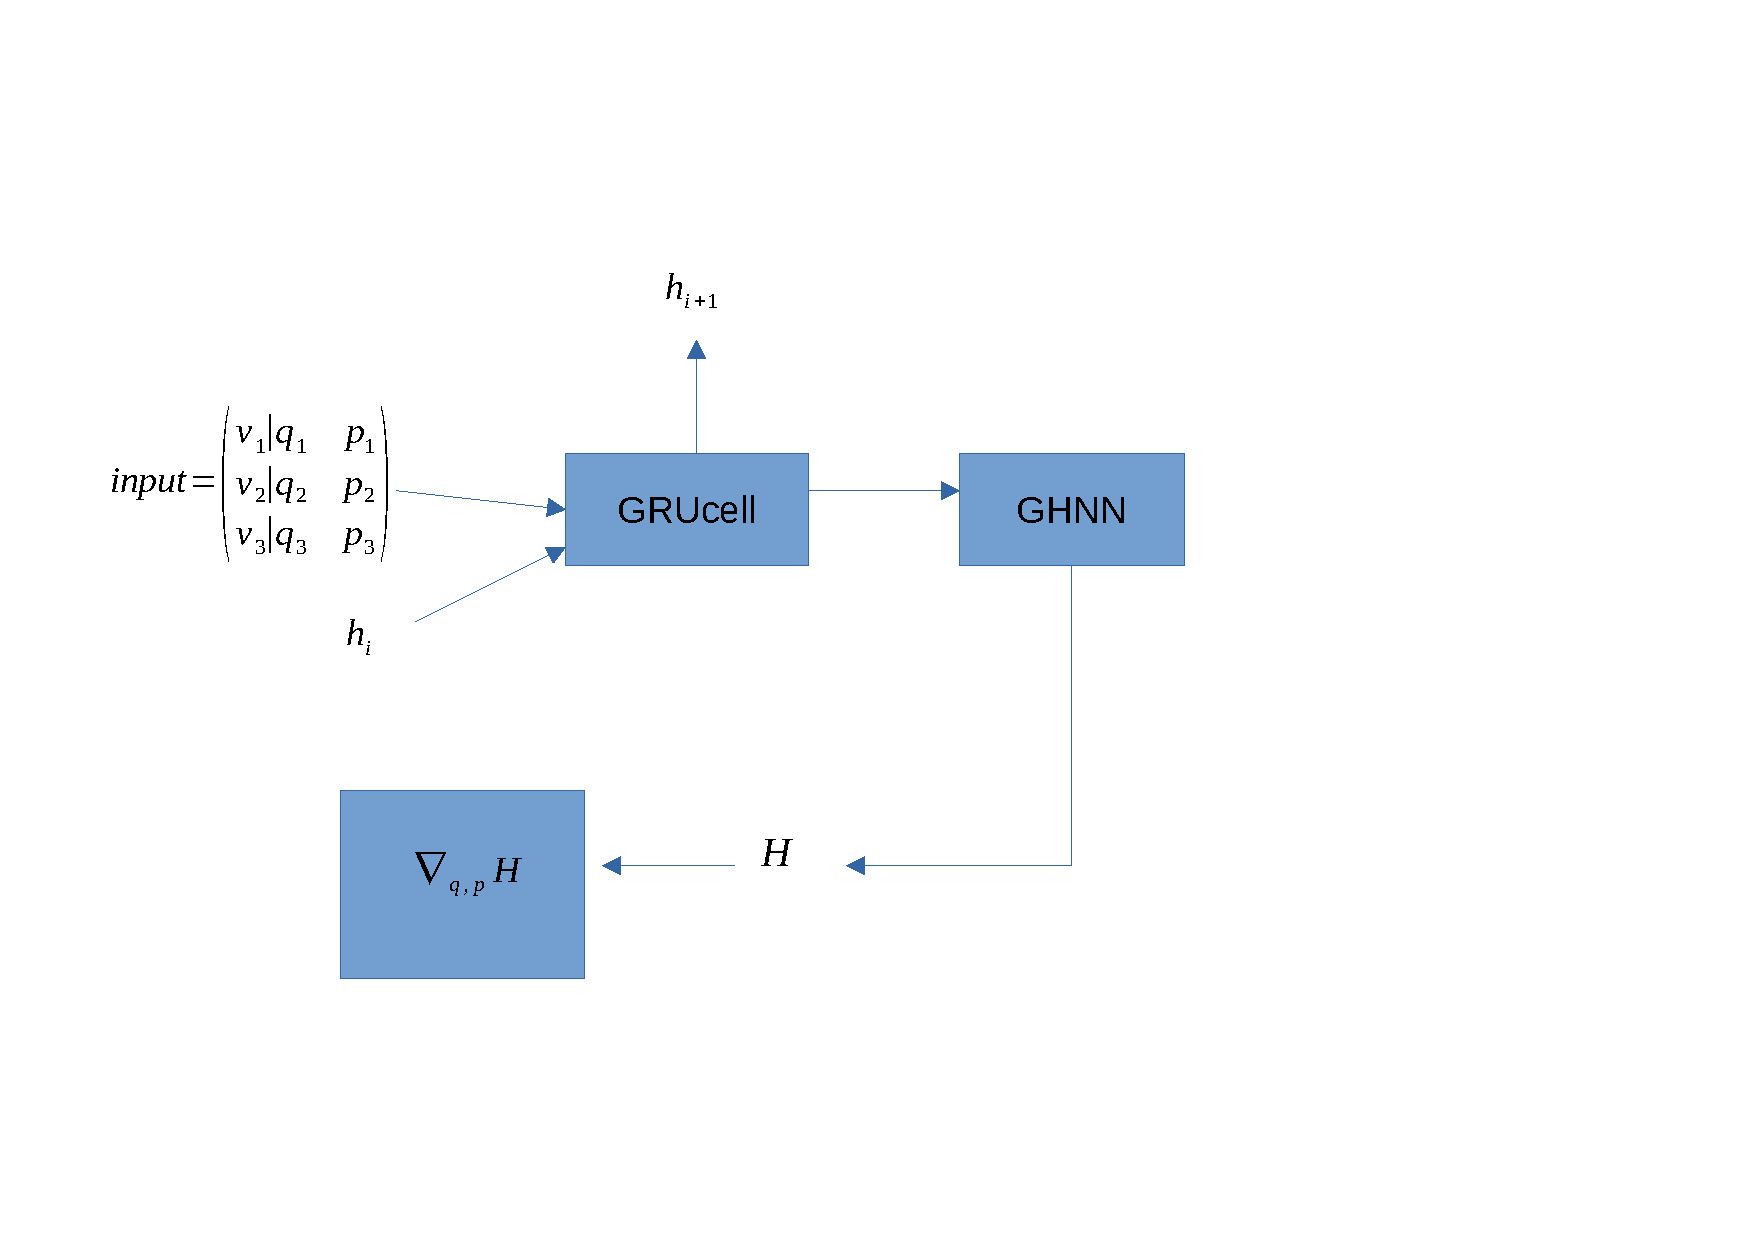
\includegraphics[width=15cm]{chapters/chapter4/GRUGHNN}
	
	\caption{Architecture of GRUGHNN}
	\label{GRUGHNN}
\end{figure}
\section{Training for Physics Informed Models based on ODE}
As we introduced the models we can observe that they are intended to be used in some ODE solver. That means that the data and our datasets are time series oriented. The specifics of time-series data are they have three dimensions which are time $t$, sample space $s$ and feature space $f$. Let us define it as $\mathcal{V}^{t,s,f}$.\\
This sample is very specific, and in case of mini-batching we can't just pick some values and make a batch, the data follow the timeflow.We need, to create the batches, specify the length of the sequence and how many sequences are in the sample. We call it \texttt{timebatch size} and \texttt{batch size}.\\
Such \texttt{time batches} we call snapshots $\mathcal{V}^{t,f}$, because it represents recorded confined sequence for one specific initial value. For example we have a sequence with 128 time points and with $\texttt{timebatch size} = 32$ we can make 96 snapshots with sequence size 32. Even if the data repeats itself it is important that we need to use many initial values as possible.\\
If we have to many samples or to big sequence we can implement \texttt{stride} technique. We specify which sequence will we recorded for our dataset. For example with \texttt{stride}=4 we specify that we want every forth inital value and its sequence recorded. Resulting in smaller dataset.\\
In case of graph batched data we need to be careful. First our sample space will change in $\mathcal{V}^{s \times n,t,f}$ where  $n$ means nodes. First we need to transform our made snapshots to graph structure, which means to place the features at their corresponding nodes and we get $\mathcal{V}^{n,t,f}$. The batching is very straight forward, it could be called "stacking the graphs". We make one big graph using $s$ times graphed independent snapshots. We call it independent because there are no edge connections between other graphs and propagating between nodes of the graphs is done in parallel.\\
In case of Hamiltonian Neural Networks and extracting a hamiltonian values of the independent graphs we suggest to unbatch it first and create a normal batch of hamiltonian values. It makes calculation of hamiltonian easier. If you calculate from the batched form, you need to be careful because the  hamiltonian can be incorrect because, we need to sum the features in every  independent graph separately.      


